%
% ------------------------------------------------------------------------------
\section{Logic-tree description}
\label{hazard:logic_tree}
A logic tree is defined in terms of three main elements:
\begin{itemize}
\item \textbf{Individual Branch}
\item \textbf{Branch Set}
\item \textbf{Branching Level}
\end{itemize}
An individual branch represent a particular realization of an epistemic uncertainty, and is therefore defined by an \textbf{uncertainty model} and an \textbf{uncertainty weight}. A branch set collects all the individual branches that describe a particular epistemic \textbf{uncertainty type}, and consequently  requires all individual branches' weights to sum to one. A logic tree structure can then be assembled by placing branch sets in a sequence, each position being represented by a branching level (see Figure \ref{fig:LogicTreeGeneralStructure}).
\begin{figure}
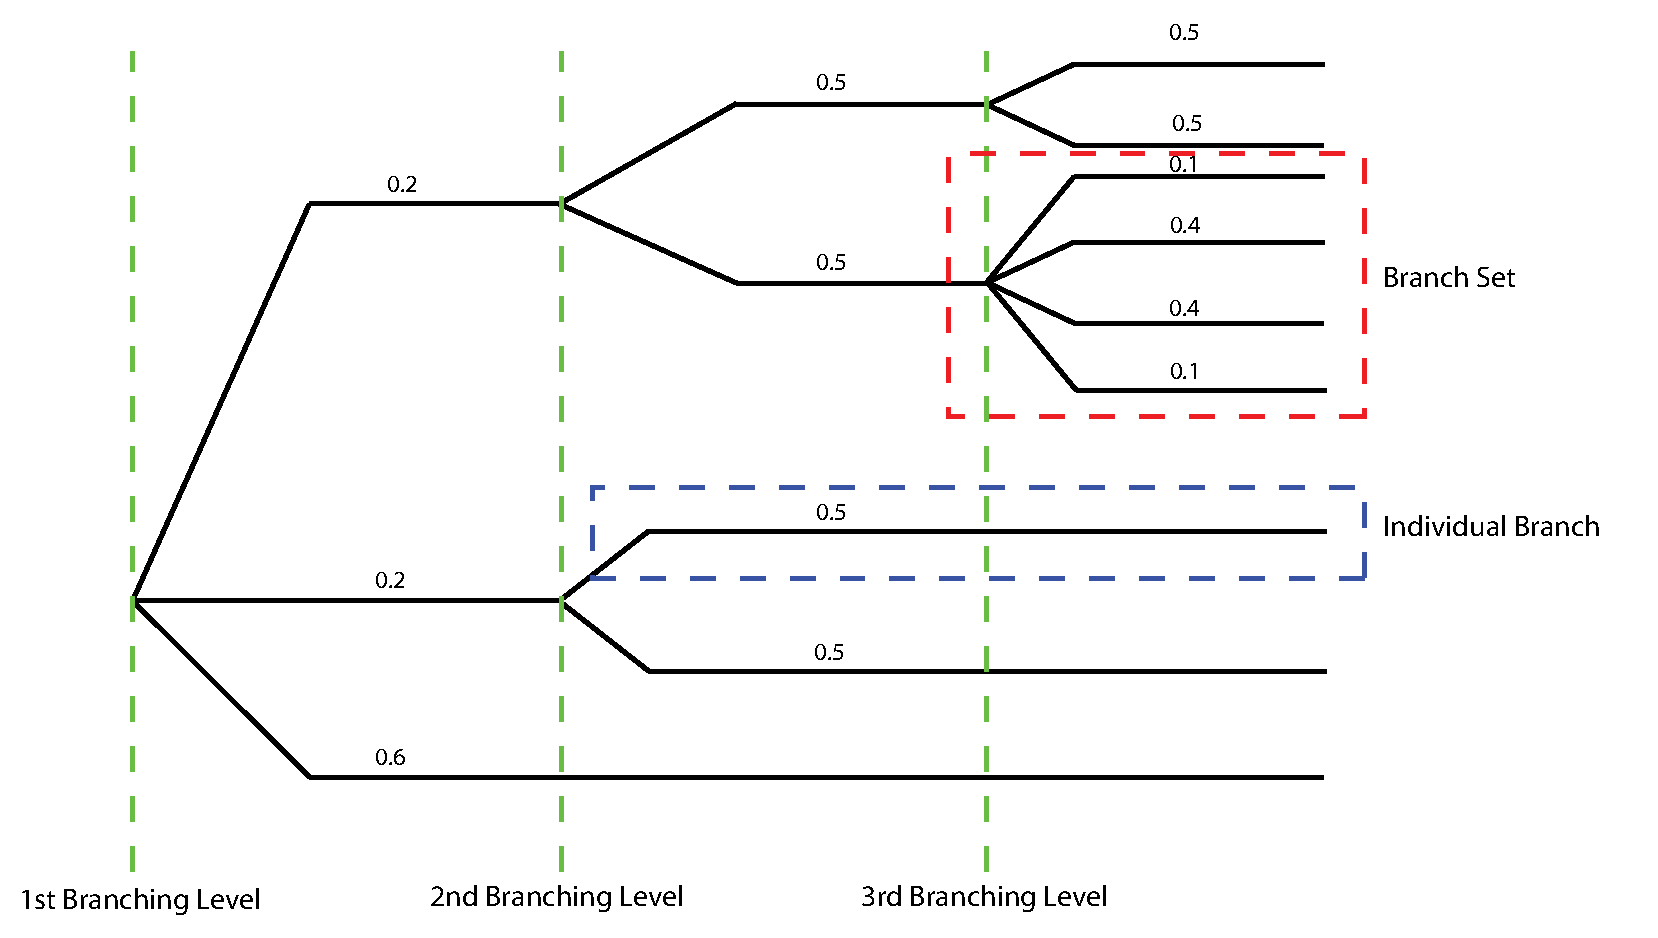
\includegraphics[width=15cm]{./Figures/Part_Hazard/LogicTreeGeneralStructure.eps}
\caption{Logic Tree data structure as defined in terms of individual branches, branch sets, and branching levels.}
\label{fig:LogicTreeGeneralStructure}
\end{figure}
The above described parameterization allows for a very general definition of a logic tree structure. For instance, a non-symmetric logic tree can be easily created by placing multiple branch sets in the same branching level, each branch set being connected to a specific branch of a branch set defined in a previous branching level.
\subsection{Source Model Logic Tree}
\label{hazard:source_model_logic_tree}
In the current version of OpenQuake, a source model logic tree can be defined according to the following schema:
\begin{itemize}
\item the 1st branching level is assumed describing one or more "alternative" initial source models.
\item subsequent branching levels define source parameters uncertainties.
\item one branch set can be defined for branching level, thus assuming symmetric logic tree definition only.
\end{itemize}
The possibility of defining multiple source models in the first branching level responds to the need of modern PSHA of considering alternative source model creation approaches (as derived by different expert opinions, data sets, modeling methodologies, for instance). Subsequent branching levels allows defining epistemic uncertainties that apply to specific parameters seismic sources depends upon. Parameter-related epistemic uncertainties are implemented as \textbf{rules}, that is as algorithms describing how a certain model parameter has to be altered. The major advantage of using a rule-based approach is that a user does not need to a provide an input file containing a source model definition corresponding to a specific epistemic uncertainty, that is instead computed and applied on the fly to the initial model. The current version of OpenQuake offers two built-in rules:
\begin{itemize}
\item Gutenberg-Richter b value uncertainties. The user can specify a set of increments (positive or negative) that are added to Guteneberg-Richter b values. Conservation of total moment rate is assumed.
\item Gutenberg-Richter maximum magnitude uncertainties. The user can specify a set of increments (positive or negative) that are added to Guteneberg-Richter maximum magnitude values. Conservation of total moment rate is assumed.
\end{itemize}
Figure \ref{fig:SourceModelLogicTree} depicts a source model logic tree that can be defined with the options currently present in OpenQuake. 
\begin{figure}
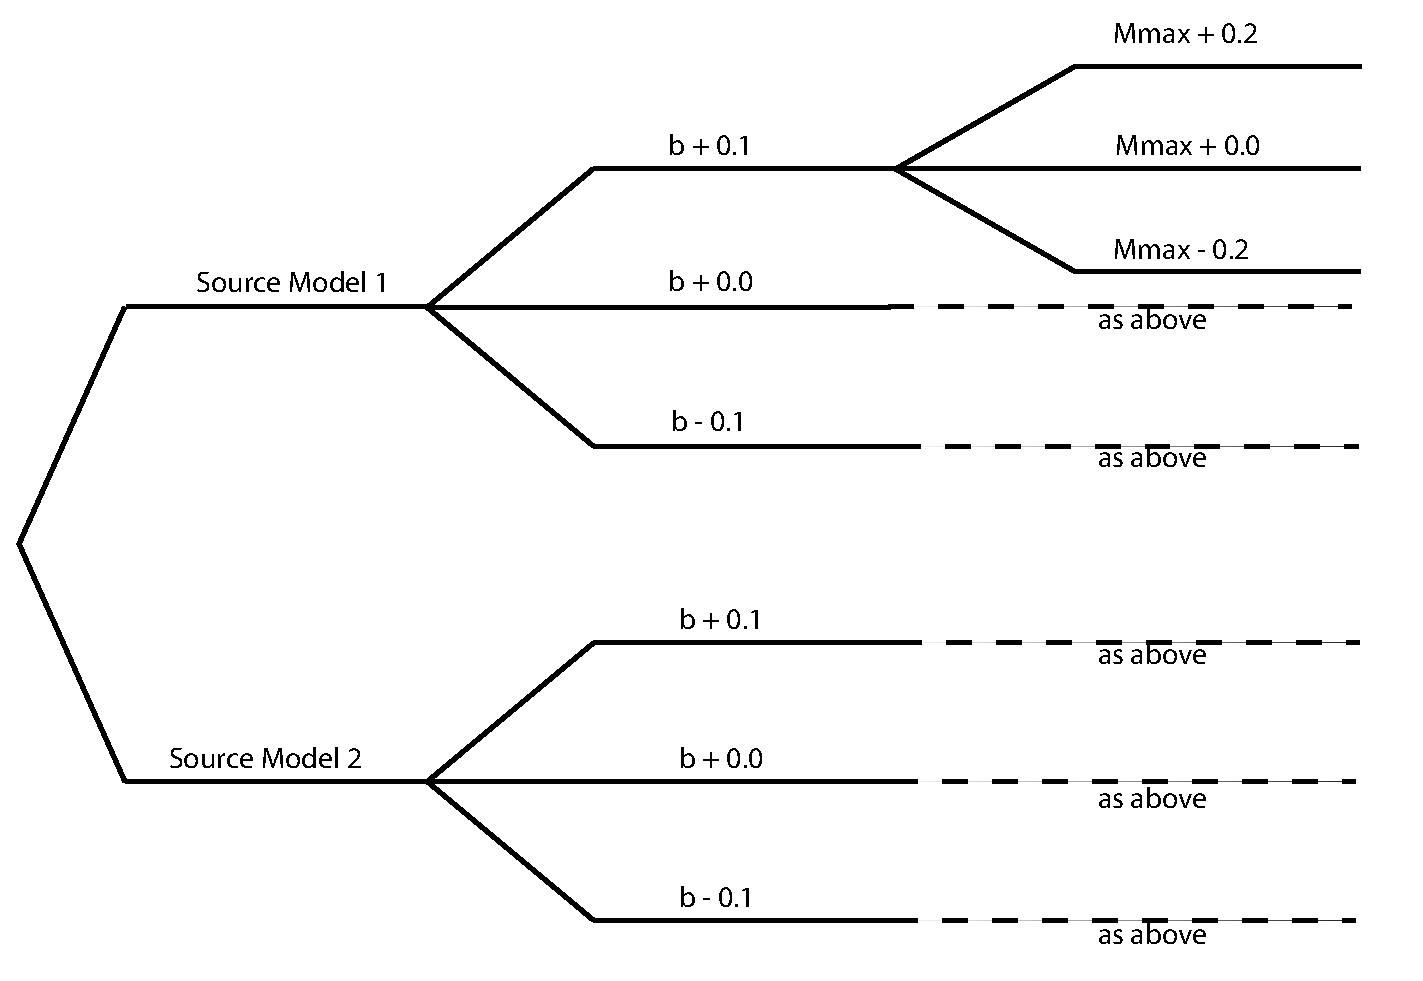
\includegraphics[width=15cm]{./Figures/Part_Hazard/SourceModelLogicTree.eps}
\caption{Example of Source Model Logic Tree. The first branching level defines two alternative source models (Source Model 1, Source Model 2). The second branching level defines uncertainties in b value (increment of 0.1, 0.0, -0.1). The third branching level defines uncertainties in maximum magnitude (increments of 0.2, 0.0, -0.2).}
\label{fig:SourceModelLogicTree}
\end{figure}
The above mentioned rules are only a sample of possible source model epistemic uncertainties, and future versions of OpenQuake will provide a broader spectrum of built-in epistemic uncertainties. Currently, rules are applied to all sources. Option to apply rules only to specific sources will be also supported in the future.
\subsection{GMPE Logic Tree}
\label{hazard:gmpe_logic_tree}
The GMPE Logic Tree allows a user to consider multiple ground motion prediction equations in the hazard modeling. Given that GMPEs are often, or can be, associated to specific tectonic region types, OpenQuake allows the definition of multiple GMPE logic trees, one for each tectonic region type considered in the source model. In the current version, a GMPE logic tree can have only one branching level, containing only one branch set, where each individual branch is associated to a specific GMPE. With the current setting, epistemic uncertainties coming from different models can be taken into account, but epistemic uncertainties inside each model cannot be captured.
Figure \ref{fig:GMPELogicTree} schematically shows GMPE logic trees that can be currently defined in OpenQuake.
\begin{figure}
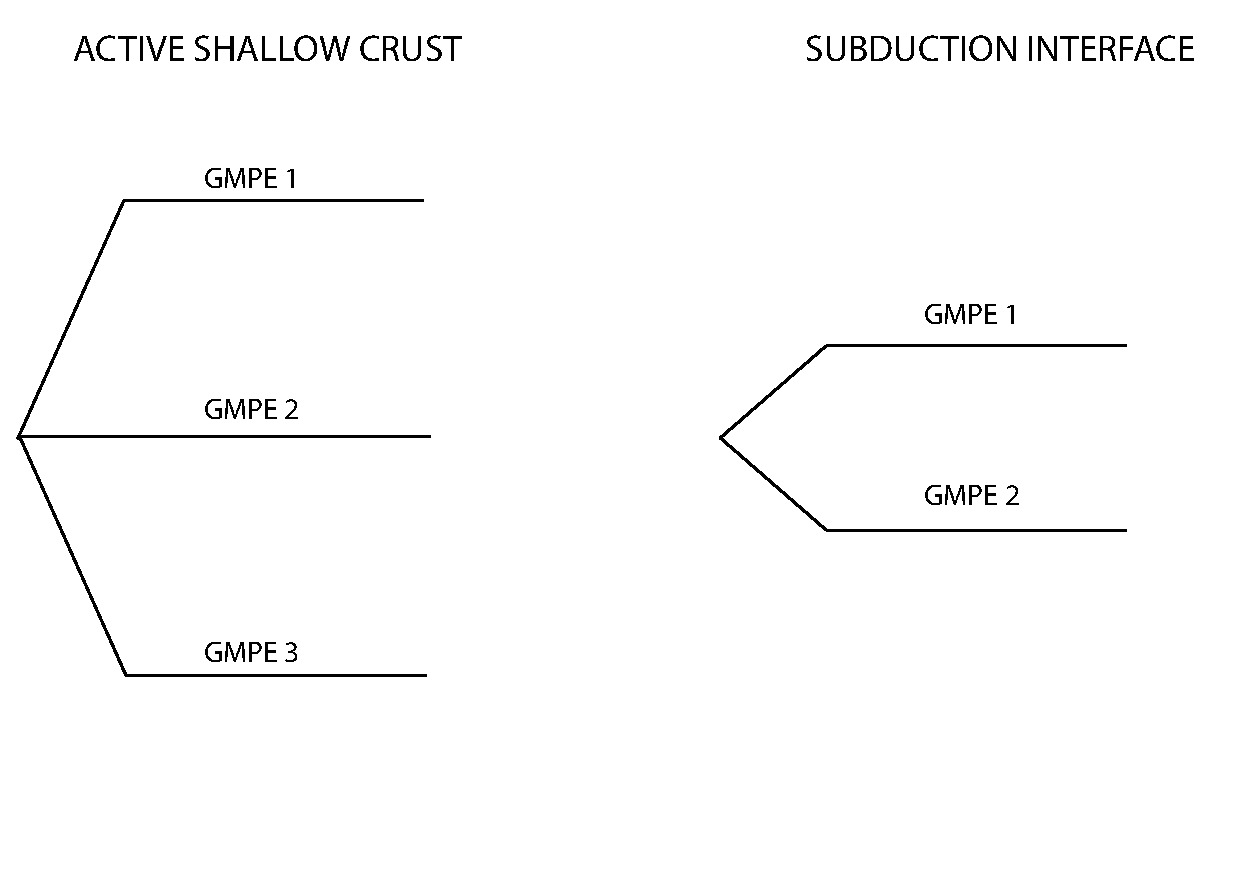
\includegraphics[width=15cm]{./Figures/Part_Hazard/GMPELogicTree.eps}
\caption{Examples of GMPE Logic Trees. One for active shallow crust (considering three GMPEs) and one for subduction interface (considering two GMPEs).}
\label{fig:GMPELogicTree}
\end{figure}



\begin{comment}
Logic-trees are a tool designed to consider in a systematic manner the 
epistemic uncertainties of models and parameters included in a hazard 
analysis.
% . . . . . . . . . . . . . . . . . . . . . . . . . . . . . . . . . . . > Figure
\renewcommand{\psedge}{\ncdiag[armA=0,angleB=180,armB=1cm]}
\begin{figure}[!hb]
%\fbox{\begin{minipage}{\textwidth}
\hfill \\
\textcolor{blue01}{\emph{Branching level definition}}: \dotfill Simple Fault 
	Dip Angle \\
\textcolor{blue01}{\emph{Branching level uncertainty type}}: \dotfill 
	Absolute values \\
\textcolor{blue01}{\emph{Applies to}}: \dotfill Simple faults \\
\textcolor{blue01}{\emph{Correlated branches}}: \dotfill Yes \\
\hfill \\
	\centering
	\begin{psTree}[treemode=R,levelsep=*2cm]
			{\Tr{ }}
		\begin{psTree}[treemode=R]{
			\Tr{\parbox[b]{4cm}{ value = 30$^\circ$ 
				\newline weight=w$_1$}}}%
		\end{psTree}%
		\begin{psTree}[treemode=R,treenodesize=1cm]{
			\Tr{\parbox[b]{4cm}{ value = 45$^\circ$ 
				\newline weight=w$_2$}}}%
		\end{psTree}%
		\begin{psTree}[treemode=R]{
			\Tr{\parbox[b]{4cm}{ value = 60$^\circ$ 
				\newline weight=w$_3$}}}%
		\end{psTree}%
	\end{psTree}%
\\ \hfill \\
%\end{minipage}} % End of fbox
\caption{Branching level description example. The upper example shows a 
branching level describing epistemic uncertainties on faults dip angle}
\label{fig:logic_tree_branching_levels}
\end{figure}
% . . . . . . . . . . . . . . . . . . . . . . . . . . . . . . . . . . . < Figure
%
\index{Logic Tree!Branching level}
In OpenQuake, the description of a logic-tree structure uses as its principal 
component a branching level where a branching level consists on (1) the 
definition of the parameter - or elements - affected by uncertainty, (2) the 
specification of the type of uncertainty (3) the listing of the - mutually 
exclusive and collectively exhaustive \citep{bommer2008} - alternative 
hypotheses and, (4) the index of the branches of the previous level - or the subset of seismic sources- to which this branching level applies.
%
\index{Logic Tree!Branch}
Each hypothesis (i.e. branch) included in a branching level has an associated value and a corresponding weight expressing - according to different interpretations available in the literature - ``probabilities or simply subjective indications of relative merit'' \citep[][page 999]{bommer2008}.

Figure \ref{fig:logic_tree_branching_levels} depicts an example of a branching level defining epistemic uncertainties on the dip angle of simple 
fault sources. In this case the possible values of the dip are specified
on each branch composing the branching level (i.e. 30, 45 and 60 degrees). This 
means that these three values are the only ones admitted for all the sources 
included in the Source Model considered in this example. 

Figure \ref{fig:logic_tree_branching_levels_1} shows a second example of a branching level defining epistemic uncertainties on the dip angle of simple fault sources. In this case the values specified for each branch aren't absolute dip angles but instead delta values to be added - or subtracted - to the initial dip value specified for each simple fault source contained in the initial source model.
% . . . . . . . . . . . . . . . . . . . . . . . . . . . . . . . . . . . > Figure
\renewcommand{\psedge}{\ncdiag[armA=0,angleB=180,armB=1cm]}
\begin{figure}
%\fbox{\begin{minipage}{\textwidth}
\hfill \\
\textcolor{blue01}{\emph{Branching level definition}}: \dotfill
	Simple Fault Dip Angle \\
\textcolor{blue01}{\emph{Branching level uncertainty type}}: \dotfill
	Relative values \\
\textcolor{blue01}{\emph{Applies to}}: \dotfill
	All previous branches \\
\textcolor{blue01}{\emph{Correlated branches}}: \dotfill Yes \\
\hfill \\
	\centering
	\begin{psTree}[treemode=R,levelsep=*2cm]
			{\Tr{ }}
		\begin{psTree}[treemode=R]{
			\Tr{\parbox[b]{4cm}{ value = -15$^\circ$ 
				\newline weight=w$_1$}}}%
		\end{psTree}%
		\begin{psTree}[treemode=R,treenodesize=1cm]{
			\Tr{\parbox[b]{4cm}{ value = 0$^\circ$ 
				\newline weight=w$_2$}}}%
		\end{psTree}%
		\begin{psTree}[treemode=R]{
			\Tr{\parbox[b]{4cm}{ value = +15$^\circ$ 
				\newline weight=w$_3$}}}%
		\end{psTree}%
	\end{psTree}%
\\ \hfill \\
%\end{minipage}} % End of fbox
\caption{Branching level description example. The upper example shows a 
branching level describing epistemic uncertainties on faults dip angle}
\label{fig:logic_tree_branching_levels_1}
\end{figure}
% . . . . . . . . . . . . . . . . . . . . . . . . . . . . . . . . . . . < Figure
%
Once two or more branching levels are defined, in flexible fashion they can be  combined (i.e. concatenated) to create an entire logic-tree structure.
	\marginpar{marco: we probably need abstract classes for all these 
	components of the LT structure}
Figure \ref{fig:logic_tree_schema} shows an example of a logic tree structure 
obtained by combining two branching levels described  in the upper part of the figure. The first branching level accounts for epistemic uncertainties connected with the dip of simple fault sources whilst the second branching level specifies the epistemic uncertainties relative to the depth to the top of rupture for (this branching level also applies to simple faults included in the model).
%
% . . . . . . . . . . . . . . . . . . . . . . . . . . . . . . . . . . . > Figure
\begin{figure}
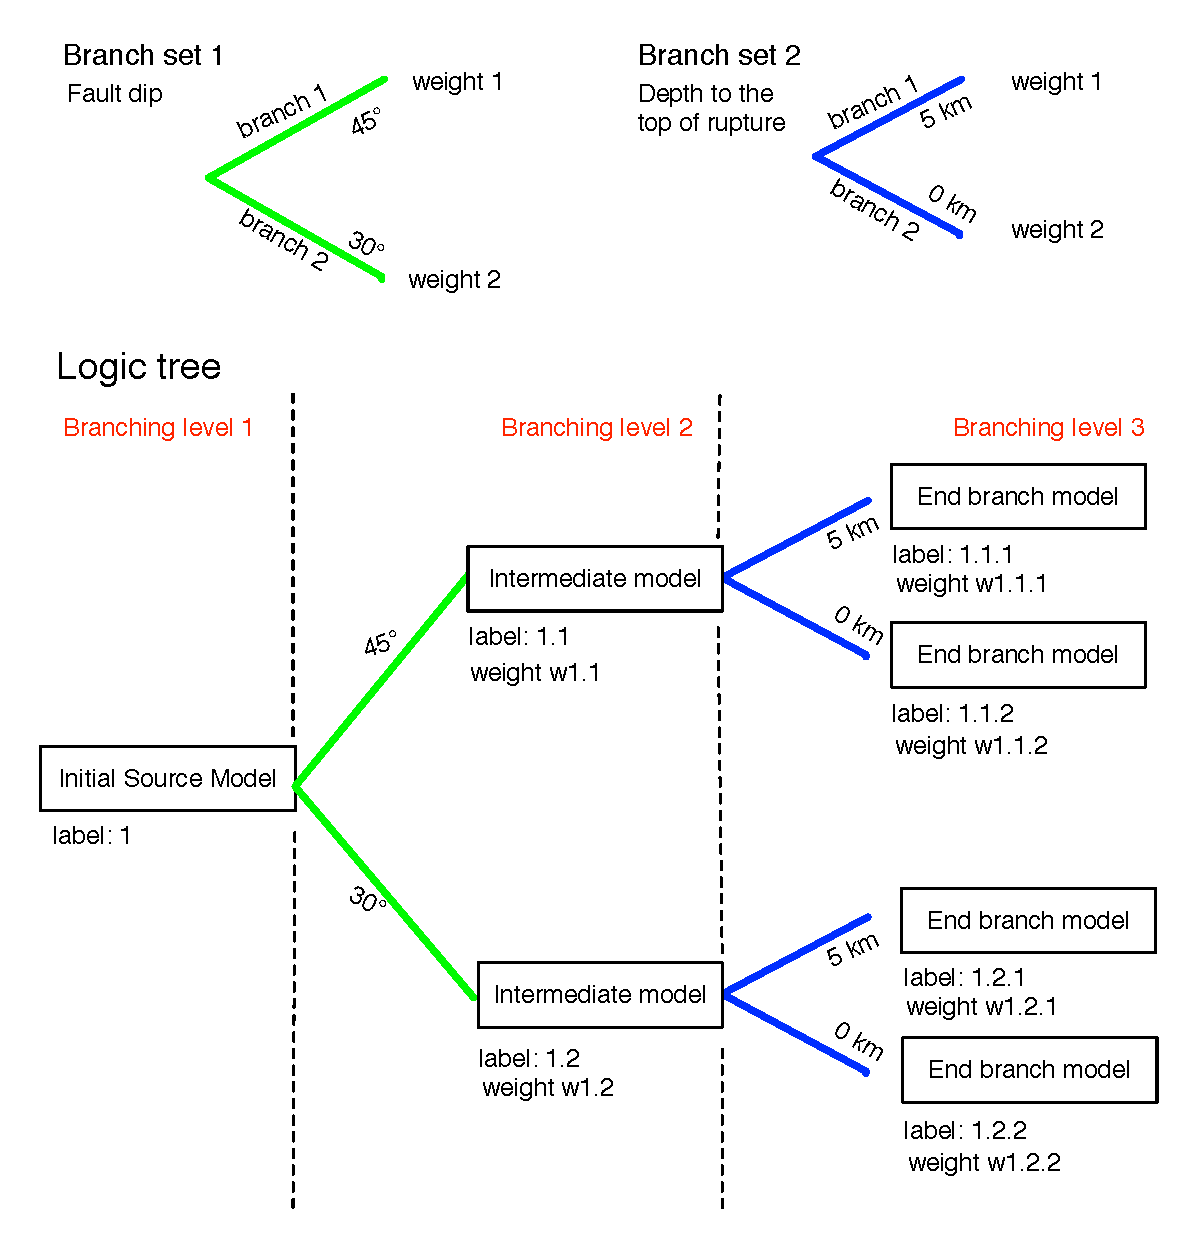
\includegraphics[width=15cm]{./Figures/Part_Hazard/logic_tree_schema.eps}
\caption{Example of a logic tree structure as defined in OpenQuake. The upper
part of the Figure depicts two branching levels.}
\label{fig:logic_tree_schema}
\end{figure}
% . . . . . . . . . . . . . . . . . . . . . . . . . . . . . . . . . . . < Figure
%
We use this logic tree description to specify the structure of the Seismic Source Logic Tree as well as for the Ground Motion Prediction Equation Logic Tree. 

%In the following paragraphs we provide a detailed description of these
%Logic Tree structures.
%%
%%  - - - - - - - - - - - - - - - - - - - - - - - - - - - - - - - - - - - - - - -
%\subsection{Seismic Source Logic Tree description and the Seismic Sources system}
%\index{Seismic Sources System}
%%
%OpenQuake uses a Seismic Source Logic Tree to describe epistemic uncertainties affecting parameters - or elements (e.g. the geometry of an area seismic source) - being part of a Seismic Source Model. 
%%
%%  - - - - - - - - - - - - - - - - - - - - - - - - - - - - - - - - - - - - - - -
%\subsection{Ground Motion Prediction Equation Logic Tree description and the GMPE System}
%%
\end{comment}
